Die Abbildung \ref{fig:TestingPyramide} ist eine Darstellung zwischen den verschiedenen Testtypen zueinander.
Die Testtypen werden in den nächsten Kapiteln beschrieben. 
Die Kategorien, in denen die Testtypen miteinander verglichen werden, sind:
\begin{itemize}
    \item Anzahl an Tests
    \item Komplexität
    \item Zerbrechlichkeit
    \item Wartungskosten
    \item Laufzeit
    \item Zeit um den Fehler zu lokalisieren
\end{itemize} 
Die Farben in der Pyramide symbolisieren die Priorisierung jedes einzelnen Testtypes.
Laut der Pyramide sollen zum Beispiel Unittests vor Integrationtests priorisiert werden.
D.h. die Integrationtests testen keine Funktionalitäten, die mit Unittests abgedeckt werden können. 


\begin{figure}[H]
    \centering
    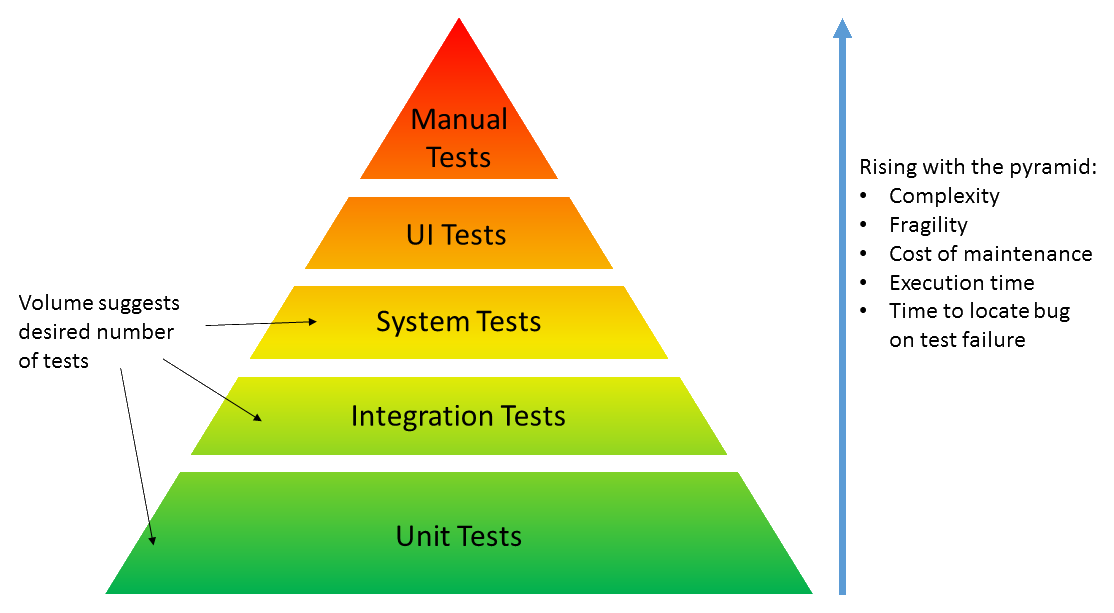
\includegraphics[width=0.8\textwidth]{Images/test_pyramid.png}
    \caption[Testing Pyramide]{Caption written below figure \footnotemark}
    \label{fig:TestingPyramide}
\end{figure}
\footnotetext{https://www.cqse.eu/de/news/blog/junit3-migration/}